\chapter{Redes \textit{ad hoc} vehiculares (VANETs)}
%-----------------------------------
%   VANETS
%-----------------------------------
\label{ch:vanets}

% En general, toda red sirve para compartir información entre dispositivos, y
% todas comparten la misma arquitectura. No obstante, la principal diferencia
% entre los distintos tipos de redes se encuentra en los protocolos de
% comunicación. Los protocolos para redes móviles son más complejos que los
% protocolos para redes de infraestructura fija. Esto es porque la comunicación
% inalámbrica tiene problemas inherentes que no se presentan en la comunicación
% alámbrica. Los protocolos de comunicación son los que se encargan de lidiar con
% estos problemas.
% 
% En este capítulo, se presenta una introducción a las VANETs, para entender qué
% dificultades presentan para el desarrollo de los protocolos de comunicación.
% También se describe el protocolo IPv6, que es el que determina la estuctura de
% los paquetes de información que circulan a través de una red, además de las
% direcciones que identifican a cada nodo. Después, se describe el problema de la
% autoconfiguración de nodos en las redes móviles, y algunos protocolos que se han
% propuesto para resolverlo. Finalmente, se presentan los diferentes enfoques de
% enrutamiento y ejemplos de protocolos de enrutamiento para redes \textit{ad
% hoc}.

Una red es un conjunto de dispositivos que están interconectados mediante
enlaces que les permiten intercambiar mensajes. Estos dispositivos, denominados
\textit{nodos} a partir de aquí, pueden ser computadoras, teléfonos,
enrutadores, o cualquier tipo de dispositivo que sea capaz de comunicarse con
los demás \cite{Marsic2013}.

La \textit{topología} de una red el conjunto de nodos que la forman y los
enlaces entre ellos \cite{Dordal2014}. La topología, por lo general, se
representa con un grafo, en el que los vértices son los dispositivos que forman
la red, y las aristas son las conexiones físicas entre ellos. En la figura
\ref{fig:topologias} se muestran dos topologías diferentes.

\begin{figure}[th]
\centering

\begin{subfigure}[b]{0.45\textwidth}
\centering
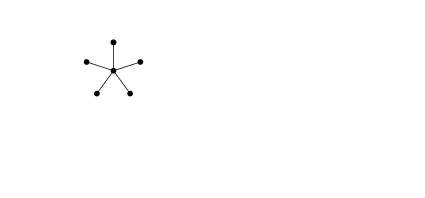
\includegraphics{topologia_estrella}
\caption[Topología de estrella.]{Topología de estrella.}
\label{fig:topologia_estrella}
\end{subfigure}
\hfill
\begin{subfigure}[b]{0.45\textwidth}
\centering
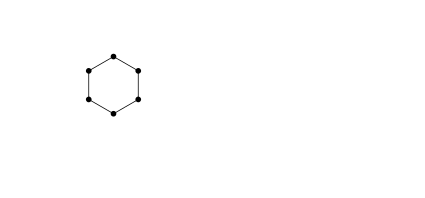
\includegraphics{topologia_anillo}
\caption[Topología de anillo]{Topología de anillo.}
\label{fig:topologia_anillo}
\end{subfigure}
\hfill
\begin{subfigure}[b]{0.45\textwidth}
\centering
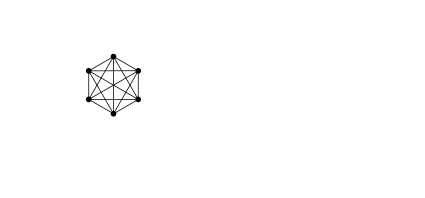
\includegraphics{topologia_malla}
\caption[Topología de malla]{Topología de malla.}
\label{fig:topologia_malla}
\end{subfigure}

\decoRule
\caption[Dos topologías diferentes]{Dos topologías diferentes.}
\label{fig:topologias}
\end{figure}

Una VANET es una red inalámbrica donde los nodos son dispositivos a bordo de
vehículos. En este documento, cuando se esté hablando de una VANET, entiéndase
``nodo'' y ``vehículo'' como sinónimos. Al tratarse de una red que no depende de
infraestructura fija, los nodos funcionan como enrutadores y \textit{hosts} al
mismo tiempo. La figura \ref{fig:vanet} muestra la representación de una VANET.

\begin{figure}[th]
\centering
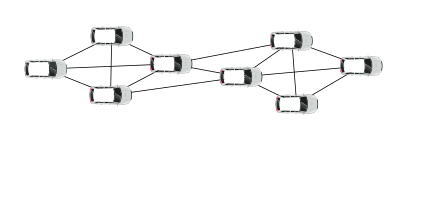
\includegraphics{vanet}
\decoRule
\caption[Red \textit{ad hoc} vehicular]{Red \textit{ad hoc} vehicular.}
\label{fig:vanet}
\end{figure}

\section{Características de una VANET}
%-----------------------------------
%   CARACTERÍSTICAS DE UNA VANET
%-----------------------------------
\label{sec:caracteristicas_de_una_vanet}

A continuación, se presentan las características que distinguen a las VANETs de
otros tipos de redes inalámbricas \cite{Meneguette2018}:

\keyword{Autoorganización} -- Al ser una red descentralizada, necesita
mecanismos que permitan a los nodos autoconfigurarse.

\keyword{Movilidad} -- Los nodos de una VANET se mueven muy rápidamente. Sin
embargo, la movilidad está restringida por la infraestructura vial, lo que hace
que sea relativamente predecible.

\keyword{Velocidad de transmisión} -- La velocidad de transmisión debe ser
rápida, debido a que dos vehículos pueden quedar fuera de alcance en pocos
segundos.

\keyword{Topología} -- Aunque la posición de los vehículos está sujeta a las
restricciones de las calles, la alta movilidad provoca cambios frecuentes en
la topología.

\keyword{Energía} -- En la mayoría de las redes inalámbricas, los nodos son
teléfonos móviles, computadoras portátiles, tabletas, u otros dispositivos que
dependen de una fuente de energía limitada. En una VANET, los nodos disponen de
una fuente de energía más abundante, por lo que también pueden contar con mayor
poder de cómputo.

\keyword{Ancho de banda} -- Los nodos pueden contar con más de un dispositivo de
comunicación, haciendo posible conectarse a diferentes redes  para lidiar con la
pérdida de conectividad y aumentar el ancho de banda.

\keyword{Fragmentación de la red} -- En ocasiones, un subconjunto de los nodos
pueden quedar aislados, debido a que su radio de comunicación no es suficiente
para alcanzar al resto de los nodos.

Las VANETs abren un gran abanico de aplicaciones para proporcionar diferentes
servicios a conductores y pasajeros. Algunas de las aplicaciones son las
siguientes \cite{Meneguette2018}:

\keyword{Aplicaciones de seguridad} -- Tienen como principal objetivo la
reducción del número de accidentes viales. Por ejemplo, advertencia cooperativa
de colisiones, asistencia para el cambio de carril, control de peligros en la
carretera, vigilancia del tráfico, notificación posterior a un accidente, etc.

\keyword{Aplicaciones de no-seguridad} -- Están destinadas a ofrecer comodidad
durante el viaje. Algunos ejemplos son notificación de servicios y páginas
amarillas, monitorización de vehículos, juegos, intercambio de información,
etc.

\section{Protocolos de comunicacion y arquitectura de red}
%-----------------------------------
%   PROTOCOLOS DE COMUNICACIÓN Y ARQUTECTURA DE RED
%-----------------------------------
\label{sec:protocolos_de_comunicacion_y_arquitectura_de_red}

Los humanos usamos protocolos para interactuar y comunicarnos en la vida
cotidiana. Por ejemplo, saludar cuando llegamos a algún lugar, presentarnos
cuando conocemos a una persona nueva, o levantar la mano para hacer una pregunta
o comentario. De la misma manera, las computadoras necesitan protocolos para
comunicarse de manera correcta. En \cite{Kurose2013} encontramos la siguiente
definición:

\begin{quotation}
Un \textit{protocolo de comunicación} define el formato y el orden de los
mensajes intercambiados entre dos o más entidades que se comunican entre sí,
así como las acciones que se realizan para la transmisión y/o recepción de un
mensaje u otro \mbox{evento}.
\end{quotation}

Una red de computadoras requiere muchos protocolos para lograr la comunicación
entre los nodos. Por ejemplo, algo tan trivial para nosotros como conectarse a
una red y consultar una página \textit{web} puede involucrar más de diez
protocolos diferentes. Sin embargo, para lidiar con esa complejidad, los
protocolos se organizan en capas, para formar lo que se conoce como la
arquitectura de red, también conocida como pila de protocolos. La arquitectura
TCP/IP\footnote{Las siglas provienen de los dos protocolos más importantes de
esta arquitectura: Protocolo de control de transmisión/Protocolo de Internet.}
(figura \ref{fig:arquitectura_tcpip}) es la más importante, ya que es sobre la
que funciona la Internet \cite{Kurose2013}.

\begin{figure}[th]
\centering
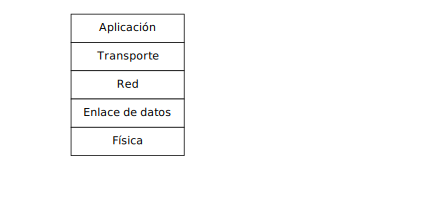
\includegraphics{arquitectura_tcpip}
\decoRule
\caption[Arquitectura TCP/IP]{Arquitectura TCP/IP.}
\label{fig:arquitectura_tcpip}
\end{figure}

Esta arquitectura se forma por cinco capas, y cada capa incluye varios
protocolos que les proporcionan servicios a los protocolos de la capa inmediata
superior. Las funciones que cumple cada una de las capas son los siguientes:

\keyword{Capa de aplicación} -- Contiene protocolos que ofrecen servicios
directamente a los usuarios. Estos servicios incluyen correo electrónico,
consulta de páginas \textit{web}, compartir archivos, telefonía, etc. Ejemplos:
HTTP, SMTP, FTP, SSH, etc.

\keyword{Capa de transporte} -- Es responsable de garantizar una transmisión
confiable de los datos, además del control de flujo de datos y el control de
congestión de la red. Ejemplos: TCP, UDP.

\keyword{Capa de red} -- Determina las rutas que deben seguir los paquetes de
información y se encarga de que cada uno siga su ruta hasta su destino. Sin
embargo, no garantiza la entrega de los paquetes. Los nodos más importantes en
esta capa son los enrutadores. Ejemplos: IP, BGP, RIP, OSPF, etc.

\keyword{Capa de enlace} -- Esta capa se encarga de las transmisiones de
paquetes entre nodos conectados directamente mediante un enlace. Dependiendo
del protocolo, puede ser un servicio confiable o no. Ejemplos: Ethernet, Wi-Fi,
Bluetooth, etc.

\keyword{Capa física} -- Convierte los paquetes en señales que se puedan
propagar por un medio físico y las transmite de un nodo a otro. Ejemplos: fibra
óptica, alambre de cobre, ondas de radiofrecuencia, etc.

Para que un protocolo pueda proporcionar su servicio a los de la capa superior,
se aplica un proceso que se conoce como encapsulamiento. Cuando el protocolo
que proporciona el servicio recibe un paquete del que lo solicita, le agrega su
propia cabecera al principio (también al final en algunos protocolos). De este
modo, cuando llega al nodo correspondiente, este extrae la cabecera para
analizarla y saber qué hacer con el paquete \cite{Kurose2013}.
